\documentclass[11pt,letterpaper]{article}
\usepackage[lmargin=1in,rmargin=1in,tmargin=1in,bmargin=1in]{geometry}
\usepackage{../style/homework}
\setbool{quotetype}{false} % True: Side; False: Under
\setbool{hideans}{false} % Student: True; Instructor: False

\usepackage{float} % Force Table Placement

% -------------------
% Content
% -------------------
\begin{document}

\homework{9: Due 02/28}{[Leonard] At least I didn't have to invent 26 dimensions just to make the math come out. [Sheldon] I didn't invent them. They are there. [Leonard] In what universe? [Sheldon] In all of them, that is the point.}{Sheldon Cooper \& Leonard Hofstadter, Big Bang Theory}

% Problem 1
\problem{10} A marketing firm is attempting to determine the effectiveness of their advertisements. After surveying 900 visitors to their clients website, 348 stated they saw an advertisement on their browser, 511 stated they saw an advertisement on their phone, and 97 said they had seen an advertisement on both. 
	\begin{enumerate}[(a)]
	\item Find the probability that a randomly selected surveyed individual saw an advertisement on their browser or phone.
	\item Find the probability that a randomly selected surveyed individual saw an advertisement only on their phone.
	\item Find the probability that a randomly selected surveyed individual had not seen an advertisement. 
	\item Find the probability that a randomly selected surveyed individual that saw an advertisement on their phone also saw an advertisement on their browser. 
	\item Find the probability that a randomly selected surveyed individual saw an advertisement only on their browser. 
	\end{enumerate} 

\sol 
\begin{enumerate}[(a)]
\item 
	\[
	P(\text{Browser or Phone})= \dfrac{348 + 511 - 97}{900}= \dfrac{251 + 97 + 414}{900}= \dfrac{762}{900} \approx 0.846667
	\] 

\item 
	\[
	P(\text{Only Phone})= \dfrac{511 - 97}{900}= \dfrac{414}{900} \approx 0.46
	\] 

\item 
	\[
	P(\text{None})= \dfrac{138}{900} \approx 0.153333
	\] 

\item 
	\[
	P(\text{Browser} \;|\; \text{Phone})= \dfrac{P(\text{Browser and Phone})}{P(\text{Phone})}= \dfrac{97}{97 + 414}= \dfrac{97}{511} \approx 0.189824
	\]

\item 
	\[
	P(\text{Only Browser})= \dfrac{348 - 97}{900}= \dfrac{251}{900} \approx 0.278889
	\]
\end{enumerate}

	\[
	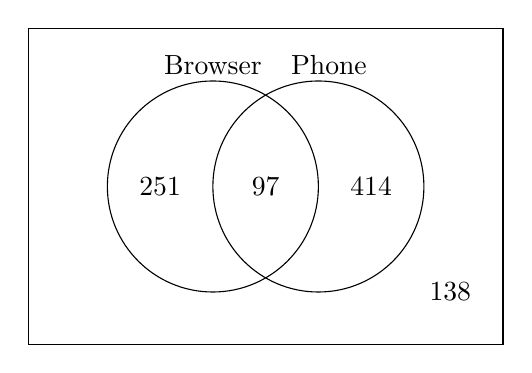
\begin{tikzpicture}[scale=0.67]
	\draw (0,0) rectangle (9,6);
	\draw (3.5,3) circle (2);
	\draw (5.5,3) circle (2);
	
	\node at (3.5,5.3) {Browser};
	\node at (5.7,5.3) {Phone}; 
	
	\node at (2.5,3) {251};
	\node at (4.5,3) {97};
	\node at (6.5,3) {414};
	\node at (8,1) {138};
	\end{tikzpicture}
	\]



\newpage



% Problem 2
\problem{10} A local college is trying to improve student academic performance at the institution. They examine the usage of various academic resources at the college, e.g. the tutoring center, library, etc. The tutoring center surveys students that use the facility over the course of the month. The survey results are shown below. \par
	\begin{table}[H]
	\centering
	\begin{tabular}{lcccc}
	 & 0 Times & 1--3 Times & $\geq$ 4 Times & Total \\ \cline{2-4}
	\multicolumn{1}{l|}{On-Campus} & \multicolumn{1}{c|}{697} & \multicolumn{1}{c|}{55} & \multicolumn{1}{c|}{12} & \multicolumn{1}{r}{764} \\
	\multicolumn{1}{l|}{Commuter} & \multicolumn{1}{c|}{457} & \multicolumn{1}{c|}{46} & \multicolumn{1}{c|}{17} & \multicolumn{1}{r}{520} \\ \cline{2-4}
	\multicolumn{1}{c}{Total} & 1,154 & 101 & 29 & 1,284
	\end{tabular}
	\end{table} \par
	
Given the data above, answer the following:
	\begin{enumerate}[(a)]
	\item Find the probability that a randomly selected student did not use the center.
	\item Find the probability that a randomly selected student is a commuter. 
	\item Find the probability that a randomly selected student did not use the center or is a commuter. 
	\item Find the probability that a randomly selected student that used the center was an on-campus student.
	\item Find the probability that a randomly selected student used the center at least four times. 
	\end{enumerate} \pspace

\sol 
\begin{enumerate}[(a)]
\item 
	\[
	P(\text{No Use})= \dfrac{1154}{1284} \approx 0.898754
	\] \pspace

\item 
	\[
	P(\text{Commuter})= \dfrac{520}{1284} \approx 0.404984
	\] \pspace

\item 
	\[
	P(\text{Not Use or Commuter})= \dfrac{1154 + 520 - 457}{1284}= \dfrac{697 + 457 + 46 + 17}{1284}= \dfrac{1217}{1284} \approx 0.947819
	\] \pspace

\item 
	\[
	P(\text{On-Campus} \;|\; \text{$\geq$ 1})= \dfrac{P(\text{On-Campus and } \geq 1)}{P(\geq 1)}= \dfrac{55 + 12}{101 + 29}= \dfrac{67}{130} \approx 0.515385
	\] \pspace

\item 
	\[
	P(\geq 4)= \dfrac{29}{1284} \approx 0.0225857
	\]
\end{enumerate}



\newpage



% Problem 3
\problem{10} A local business is analyzing their sales of one of their more popular products---the Franley cup. They place the cup on sale a mere 8\% of the time. If the cup is on sale, the business sells out of them 83\% of the time. Otherwise, they sell out of the cup only 39\% of the time. 
	\begin{enumerate}[(a)]
	\item What percentage of the time does the business sell out of the cup?
	\item What percentage of the time does the business either place the cup on sale or sell out of the cup?
	\item What percentage of the time does the company not sell out of the cup?
	\item If the company sold out of the cup, what is the probability that the cup was on sale?
	\item What percentage of the time does the company not put the cup on sale but sell out of it anyway?
	\end{enumerate} 

\sol 
\begin{enumerate}[(a)]
\item 
	\[
	P(\text{Sell Out})= 0.0664 + 0.3588= 0.4252
	\] \pspace

\item 
	\[
	P(\text{Sale or Sell})= 0.0664 + 0.0136 + 0.3588= 0.4388
	\] \pspace

\item 
	\[
	P(\text{Not Sell})= 0.0136 + 0.5612= 1 - P(\text{Sell})= 1 - = 1 - 0.4252= 0.5748
	\] \pspace

\item 
	\[
	P(\text{Sale} \;|\; \text{Sold})= \dfrac{P(\text{Sale \& Sold})}{P(\text{Sold})}= \dfrac{0.0664}{0.0664 + 0.3588}= \dfrac{0.0664}{0.4252}= 0.156162
	\] \pspace

\item 
	\[
	P(\text{Sell} \;|\; \text{Not Sale})= \dfrac{P(\text{Sell \& Not Sale})}{P(\text{Not Sale})}= \dfrac{0.3588}{0.3588 + 0.5612}= \dfrac{0.3588}{0.92}= 0.39
	\] 
\end{enumerate} \vfill

		\[
		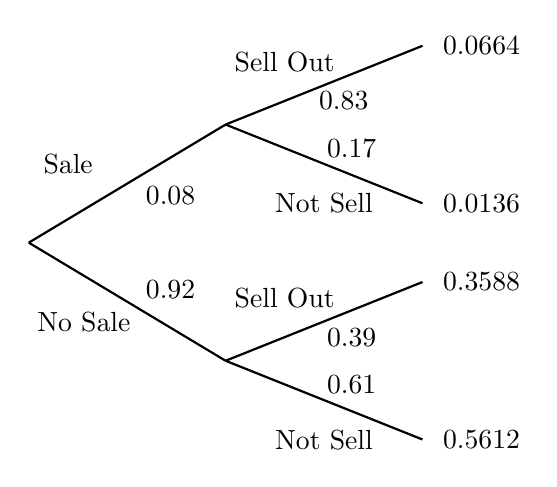
\begin{tikzpicture}[scale= 1.0]
		\def\FirstUpLabel{Sale}
		\def\FirstDownLabel{No Sale}
		\def\SecondUpLabel{Sell Out}
		\def\SecondDownLabel{Not Sell}
		\def\Up{$0.08$}
		\def\Down{$0.92$}
		\def\UpUp{$0.83$}
		\def\UpDown{$0.17$}
		\def\DownUp{$0.39$}
		\def\DownDown{$0.61$}
		\def\first{$0.0664$}
		\def\second{$0.0136$}
		\def\third{$0.3588$}
		\def\fourth{$0.5612$}
		
		\node at (0.5,1) {\FirstUpLabel};	
		\node at (0.7,-1) {\FirstDownLabel};	
		\node at (1.8,0.6) {\Up};
		\node at (1.8,-0.6) {\Down};
		\draw[thick] (0,0) -- (2.5,1.5);
		\draw[thick] (0,0) -- (2.5,-1.5);
		
		\node at (3.25,2.3) {\SecondUpLabel};
		\node at (3.75,0.5) {\SecondDownLabel};
		\node at (4,1.8) {\UpUp};
		\node at (4.1,1.2) {\UpDown};
		\node at (5.75,2.5) {\first};
		\node at (5.75,0.5) {\second};
		\draw[thick] (2.5,1.5) -- (5,2.5);
		\draw[thick] (2.5,1.5) -- (5,0.5);

		\node at (3.25,-0.7) {\SecondUpLabel};
		\node at (3.75,-2.5) {\SecondDownLabel};
		\node at (4.1,-1.2) {\DownUp};
		\node at (4.1,-1.8) {\DownDown};
		\node at (5.75,-0.5) {\third};	
		\node at (5.75,-2.5) {\fourth};	
		\draw[thick] (2.5,-1.5) -- (5,-0.5);
		\draw[thick] (2.5,-1.5) -- (5,-2.5);
		\end{tikzpicture}
		\]


\end{document}